\section{Background}

There are a number of models that can be used for bus arrival prediction, but there are four main models that are most widely used \cite{dynamic-gps}. They are as follows: 
\begin{itemize}
    \item \textbf{Historical average models}: Also known as simple forecasting, these models make use of historical bus arrival and travel times to predict the arrival time of buses. The algorithms tend to be fairly simple and are not dynamic in nature. On its own, performance could be fairly weak, due to the unreliability of traffic conditions and other factors that vary over time. 
    \item \textbf{Regression models}: These models are a form of predictive technique, which can be used to investigate the relationship between factors that affect bus arrival times (predictors) and bus arrival times (target) \cite{regression-techniques}. This technique will help to see which factors are more or less important. For example, Patnaik et al. used regression models to discover that "weather variables were not among the significant factors for estimating arrival times" \cite{apc-estimation}. 
    \item \textbf{Kalman Filtering models}: The Kalman filter is one of the optimal solutions for tracking and data prediction tasks \cite{kalman-mit}. These models are a dynamic estimation technique that have been used fairly frequently in bus delay predictions.
    \item \textbf{Machine Learning models}: These models have been widely used in research to try to improve public transportation. This project will look particularly at Artificial Neural Networks (ANNs), which are suited towards more complex and noisy data and finding non linear relationships between dependent and independent variables \cite{dynamic-gps}. 
\end{itemize}

I am not planning on exploring Kalman models any further as a model for predicting bus arrival times. This is because I think that if I include Kalman models, I will have insufficient time to properly refine all the models. I would rather have a smaller number of highly optimised models, rather than a larger number of very simple or unoptimised models.

\subsection{Historical Average Models}
\label{section:historical-avg-models-research}

\subsubsection{Forecasting}
Forecasting is an important aid to effective and efficient planning. Statistical forecasting typically refers to the use of statistics on historical data to project what could happen in the future \cite{what-is-forecasting}. The effectiveness of forecasting as a method depends on several factors including how well we understand the factors that contribute to an event, how much data is available and whether the forecasts can affect the thing we are trying to forecast \cite{forecasting-book}. A good forecast should capture the genuine patterns and relationships which exist in the historical data, but do not replicate past events that will not occur again. In the case of historical bus data, the data collected will be gathered at regular intervals over time, and therefore, can be seen as time series data. In this way, quantitative forecasting can be applied because it is reasonable to assume that some aspects of the past patterns will continue into the future.

\subsubsection{Methods}

When forecasting time series data, the aim is to estimate how the sequence of observations will continue into the future. The simplest time series forecasting methods only use information on the variable to be forecast without attempting to discover the factors that could affect its behaviour. Therefore, these methods will extrapolate trends and seasonal patterns, but will ignore other information. For example, when forecasting bus arrival times, we would look at historical information on bus delays, but would ignore factors such as traffic conditions or weather conditions. \\

Some of the most common simple forecasting methods are listed below \cite{forecasting-book}:

\begin{itemize}
    \item \textbf{Mean Method}: All the future forecast values are equal to the average of the historical data. This method is optimal when data has a fairly steady value and does not change much over time.
    \item \textbf{Naive Method}: All the future forecast values are equal to the value of the last observation. This method is optimal when data follows a random walk.
    \item \textbf{Seasonal Naive Method}: Each forecast value is set to be equal to the last observed value from the same season of the year, for example from the same month of the previous year or the same quarter of the previous year. This method tends to perform better than a simple naive method, especially when the historical data has a clear seasonal trend. 
    \item \textbf{Drift Method}: This method is a variation of the naive method. The forecast values increase or decrease over time and the amount of change over time is called the drift. This drift is set to be the average change seen in the historical data. This method is equivalent to drawing a straight line between the first and last observations and extrapolating it into the future. 
\end{itemize}

It can be seen in Figure \ref{fig:forecasting} that both the \textit{mean} and \textit{naive} methods result in flat line forecasts, and therefore, would not be particularly suitable for bus arrival predictions because research has shown that for different time periods, the trends in delay times vary \cite{dynamic-gps}, \cite{ann-prediction}, \cite{smart-public-transport}. However, a slight variation on the mean and naive method that essentially combines the two methods, where the model takes the average of the last two or three bus travel times for each forecast, is much more likely to provide a better estimate. This is because this method will use historical results that should theoretically be in the same time period (or clustering) as the current time to be forecast. This method will also avoid going too far into the past and using data that may not be relevant. Figure \ref{fig:forecasting} also shows that the \textit{seasonal naive} method results in an oscillating prediction. Since there is reason to believe that historical data on bus delay times show an up and down trend, the seasonal naive method could also be an equally suitable model to use.

\begin{figure}[H]
\begin{center}
    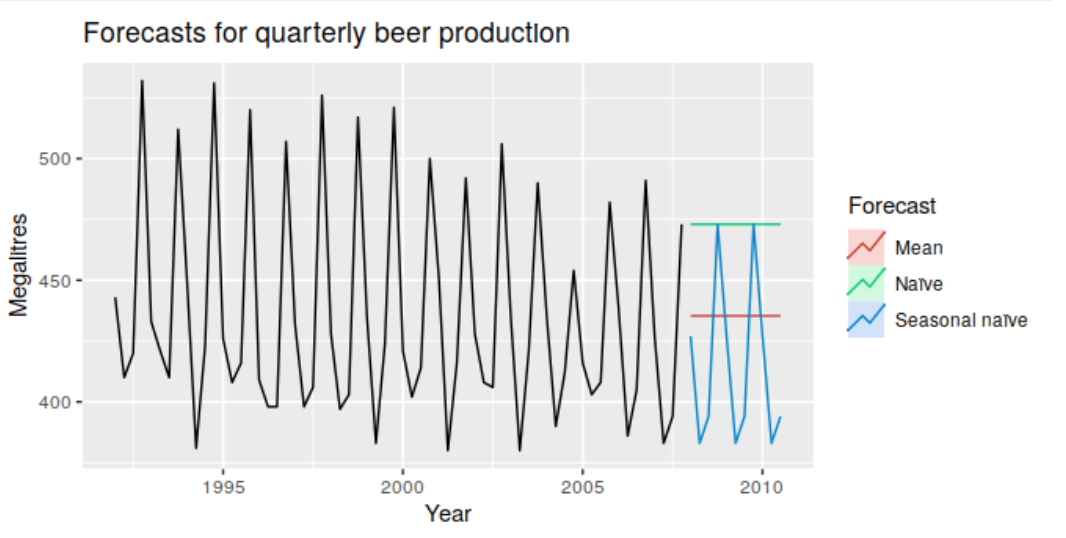
\includegraphics[width=\textwidth]{Images/forecasting-beer-prod.png}
    \caption{Example of the mean, naive and seasonal naive methods applied to quarterly beer production data, original image from \cite{forecasting-book}}
    \label{fig:forecasting}
\end{center}
\end{figure}

\subsubsection{More Complex Methods?}

Worth adding more complex methods? Or nah.

\subsubsection{Measuring Success}

Explained variance score, mse?

\subsection{Regression Models}
\label{section:regression-models-research}

Regression is a form of statistical modelling that investigates the relationship between a dependent (target) and independent (predictor) variable \cite{regression-techniques}. When performing statistical modelling, we observe some data $y$, known as the dependent variable, and interpret each data point as a realisation of some random variable $Y$ \cite{m2s2-notes}. A statistical model is a specification of the distribution of $Y$ up to an unknown parameter $\theta$. Often $y = (y_1, y_2, ..., y_n) \in \mathbb{R} ^ n$ is a vector and $Y = (Y_1, ..., Y_n)$ is a random vector. The distribution of $Y_1, ..., Y_n$ may depend on (non random or deterministic) quantities $x_1, ..., x_n$ known as covariates or predictors. 

\subsubsection{Simple Linear Regression and Multiple Regression}

In the simplest case, the regression model allows for a linear relationship between the observable variable $Y$ and a single predictor variable $x$ (Equation \ref{eq:lin-reg}): 

\begin{equation}
    Y_t = \beta_1 + x_i\beta_2 + \epsilon_t, t = 1, ..., n
    \label{eq:lin-reg}
\end{equation}

where $Y_t$ is the outcome or observable random variable, $x_t$ is the covariate constant, $\beta_0$ and $\beta_1$ denote the intercept and slope of the line respectively and $\epsilon_t$ are iid (independent and identically distributed) errors. $E(\epsilon_t) = 0$, $Var(\epsilon_t) = \sigma^2$ for $t = 1,...n$. $\sigma^2 > 0$ is also unknown. The errors are not observable and can be thought of as the deviation from the underlying straight line model, capturing anything that may affect $Y_t$ other than $x_t$ \cite{forecasting-book}. Figure \ref{fig:lin-reg} visualises the linear relationship as defined in Equation \ref{eq:lin-reg}.

\begin{figure}[H]
\begin{center}
    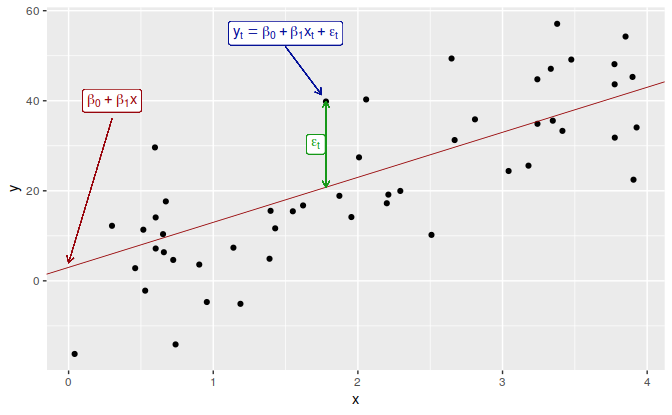
\includegraphics[width=\textwidth]{Images/linear-regression.png}
    \caption{Linear Regression, original image from \cite{forecasting-book}}
    \label{fig:lin-reg}
\end{center}
\end{figure}

When there are two or more predictor variables, the model is called a multiple regression model. The general formulation in a linear model is shown in Equation \ref{eq:multi-regression}:

\begin{equation}
    Y = \mathbf{X}\beta + \epsilon
    \label{eq:multi-regression}
\end{equation}

where $Y$ is an n-dimensional random vector (observable), $\mathbf{X} \in \mathbf{R} ^{n \times p}$ is a known matrix (often called the `design matrix'), $\beta \in \mathbf{R}^p$ is an unknown parameter and $\epsilon$ is an n-variate random vector (not observable) with $E(\epsilon) = \mathbf{0}$. The $\beta$ coefficients essentially measure the effect of each predictor after taking into account the effects of all the other predictors in the model. \\

When we use a linear regression model, we make the following assumptions.

\begin{itemize}
    \item The model is a reasonable approximation to reality, that is, the relationship between the forecast variable and the predictor variable satisfies this linear equation.
    \item We make the following assumptions about the errors:
    \begin{itemize}
        \item they have a mean of zero; otherwise the predictions will be systematically biased.
        \item they are not autocorrelated; otherwise the predictions will be inefficient.
        \item they are unrelated to the predictor variables; otherwise there would be more information that should be included as a predictor variable.
    \end{itemize}
    \item Each predictor $x$ is not a random variable.
\end{itemize}

\subsubsection{Ridge Regression? Piecewise Linear Regression?}

The data isn't particularly linear, so some other regression model?

\subsubsection{Least Squares Estimation}

Least squares estimation is a method of estimating parameters by minimising the squared discrepancies between observed data and their expected values \cite{least-squares-estimation}. Choose $\beta$ to minimise Equation \ref{eq:least-squares}:

\begin{equation}
    S(\beta) = \sum_{i=1}^n(Y_i - \sum_{j=1}^pX_{ij}\beta_j)^2 = (\mathbf{Y} - X\beta)^T(\mathbf{Y} - X\beta)
    \label{eq:least-squares}
\end{equation}

where as before, $Y$ is an n-dimensional random vector, $\mathbf{X} \in \mathbf{R} ^{n \times p}$ is a known matrix and $\beta \in \mathbf{R}^p$ is an unknown parameter. We denote the the estimated value that gives the best fit to the data of $\beta$ by $\hat \beta$.

\subsubsection{Measuring Success}

RMSE, MSE, R2-Score, MAE \\

The standard error is the equal to the standard deviation, which would be obtained from repeatedly estimating the $\beta$ coefficients on similar data sets. This gives a measure of the uncertainty in the estimated $\beta$ coefficient. \\

The p-value is the probability of the estimated $\beta$ coefficient being as large as it is if there was no real relationship between the forecast variable and the corresponding predictor. This is particularly useful when studying the effect of each predictor, and can be used as another way of seeing which parameter to use in the models and which to discard. \\ 

A common way to summarise how well a linear regression model fits the data is via the coefficient of determination (Equation \ref{eq:r-squared}:

\begin{equation}
    R^2 = \frac{\sum(\hat y_t - \bar y)^2}{\sum(y_t - \bar y)^2}
    \label{eq:r-squared}
\end{equation}

where the summations are over all the observations, $\hat y_t$ are the predicted values, $y_t$ are the observed values and $R^2$ is bounded between 0 and 1. Although this is a way of measuring `goodness-of-fit', validating the performance of a model against a test set is much better than measuring the $R^2$ value on the training data \cite{forecasting-book}. \\

The differences between the observed $y$ values and the corresponding fitted $\hat y$ values are known as residuals. To detect problems with a model, we can plot standardised residuals against some each of the predictor variables. We expect the residuals to be randomly scattered without showing any systematic pattern because a pattern would indicate a nonlinear relationship between the variables. If the model is correct then the resulting plot should just show `noise' with no distinct patterns. 

\subsubsection{Outliers}

An outlier is an observation that does not conform to the general pattern of the rest of the data. Observations that have a large influence on the estimated coefficients of a regression model are called influential observations. If an observation has been identified as a likely outlier, it is important to try and analyse why it is the case, as outliers can arise from incorrect data collection or can be an indication of the underlying model being unsuitable \cite{forecasting-book}, \cite{m2s2-notes}. Figure \ref{fig:outlier} is an example showing how an outlier can affect predictions. The red line is the regression line fitted to the data including the outliers, the black line is the regression line fitted to the data without the outlier. It can be seen that the gradient of the 2 lines are not the same and therefore, the models would give differing predictions.  

\begin{figure}[H]
\begin{center}
    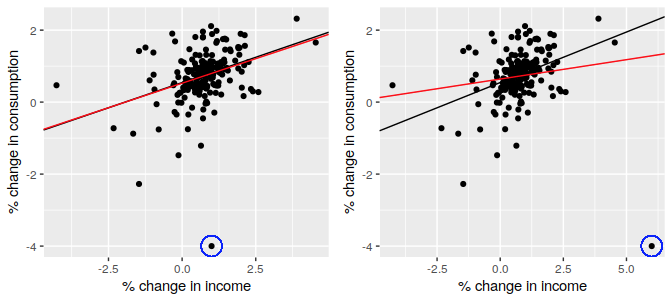
\includegraphics[width=\textwidth]{Images/outlier-analysis.png}
    \caption{Example showing how an outlier can affect predictions, original image from \cite{forecasting-book}}
    \label{fig:outlier}
\end{center}
\end{figure}

\subsection{Kalman Filtering Models}
\label{section:kalman-models-research}

Kalman filtering is an algorithm that provides estimates of some unknown variables, given the measurements observed over time \cite{kalman-korean}. The algorithm is unusual in that it consists of two processes, the prediction process and the measurement process, that work recursively \cite{kalman-malay}.  \\

The Kalman filtering algorithm starts in the prediction process and estimates the prediction state based on the derived state space equation (Equation \ref{eq:kalman}). This stage covers the prediction of the a priori state and a priori error covariance. The process model defines the evolution of the state from time $k-1$ to time $k$ as:

\begin{equation}
\label{eq:kalman}
    x_k = Fx_{k-1} + Bu_{k-1} + w_{k-1}
\end{equation}

where $F$ is the state transition matrix applied to the previous state vector $x_{k-1}$, $B$ is the control input matrix applied to the optional control vector $u_{k-1}$, and $w_{k-1}$ is the process noise vector that is assumed to be zero-mean Gaussian with covariance $Q$, i.e. $w_{k-1} \sim N(0, Q)$. The next stage is the measurement process (Equation \ref{eq:kalman-2}), which covers the calculation of the optimal Kalman gain, updating the a posteriori estimation state and the a posteriori error covariance. The measurement model describes the relationship between the state and the measurement at the current time step $k$ as:

\begin{equation}
\label{eq:kalman-2}
    z_k = Hx_k + v_k
\end{equation}

where $z_k$ is the measurement vector, H is the measurement matrix and $v_k$ is the measurement noise vector that is assumed to be zero-mean Gaussian with covariance R, i.e. $v_k \sim N(0, R)$ \\

The Kalman Filter provides estimates of $x_k$ given the initial estimate $x_0$, the series of measurements $z_1$, ..., $z_k$ and the information described by $F, B, H, Q$ and $R$. \\

\subsection{Machine Learning Models}
\label{section:ml-models-research}

Explore normal neural networks or other machine learning techniques before deciding immediately on ANNs.

(Feed-forward) Artificial Neural Networks (ANNs) are a type of machine learning inspired by real world biological neurons. 

\subsubsection{Perceptrons}

An ANN has a collection of nodes called artificial neurons, the most common type of which is called a perceptron \cite{methods-for-ds-slides}, \cite{neural-networks-book}. A perceptron takes $m + 1$ inputs $x_{i\in{0,...,m}}$ with $m + 1$ weights $w_{i\in{0,...,m}}$ and produces a single binary output $y$. Weights are real numbers expressing the importance of the respective inputs to the output. So a perceptron's output, 0 or 1, is determined by whether the weighted sum is less than or greater than some threshold value (Equation \ref{eq:perceptron}).

\begin{equation}
    output = 
    \begin{cases} 
        0 if \sum_jw_jx_j \leqslant threshold \\
        1 if \sum_jw_jx_j > threshold
    \end{cases}
    \label{eq:perceptron}
\end{equation}

By varying the weights and the threshold, we can get different models of decision making. We set the bias of a perceptron to be $w_0$ and set $x_0 = 1$. The bias is a measure of how easy it is to get the perceptron to output a 1. The perceptron can be `activated' using a non linear activation function $g$, allowing us to approximate arbitrarily complex function. There are a number of different activation functions, with some common ones including the \textit{Sigmoid} function: $ \sigma(x) = \frac{1}{1 + e^{-x}} $ and the \textit{ReLU} function: $ max(0, x) $. Figure \ref{fig:perceptron} shows a single perceptron with 3 input neurons ($x_0$ = 1 and $w_0$ is the bias) and output $\mathbf{\hat y}$.

\begin{figure}[H]
\begin{center}
    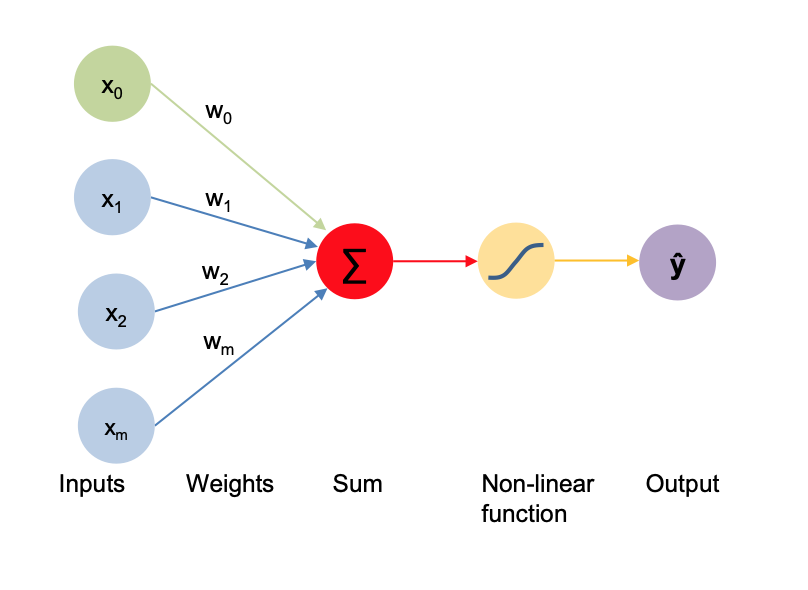
\includegraphics[scale=0.8]{Images/perceptron-forward-prop.png}
    \caption{The Perceptron: forward propagation, original image from \cite{methods-for-ds-slides}}
    \label{fig:perceptron}
\end{center}
\end{figure}

\subsubsection{Neural Network Architecture}

ANNs consists of stacking neurons into layers, with different layers performing transformations on their inputs. These models are called feed-forward because information flows from input $x$ to output $y$ without any feedback connections in which outputs of the model are fed back into itself, i.e. information always travels forward \cite{deep-learning-book}. Figure \ref{fig:nn-architecture} shows a fully connected neural network with a single layer. The leftmost layer is called the input layer, the rightmost layer is called the output layer and the middle layers are called hidden layers. Neural networks with multiple hidden layers are sometimes called multi-layer perceptrons.

\begin{figure}[H]
\begin{center}
    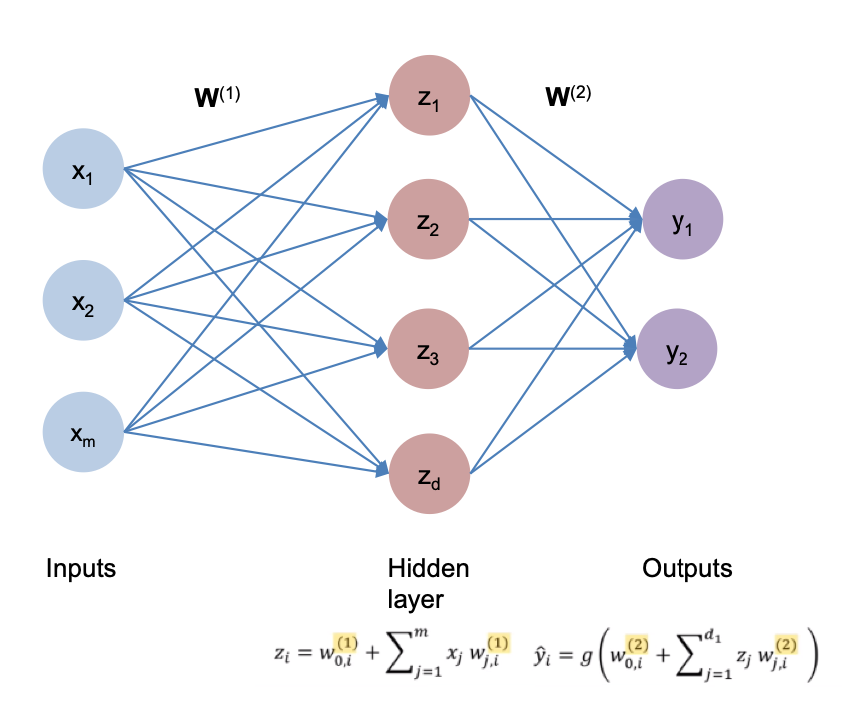
\includegraphics[scale=0.8]{Images/single-layer-nn.png}
    \caption{Fully connected single layer neural network, original image from \cite{methods-for-ds-slides}}
    \label{fig:nn-architecture}
\end{center}
\end{figure}

\subsubsection{Back Propagation}

Content

\subsubsection{Loss Functions}

Loss functions, also known as objective functions cost functions empirical risk, are used to train the neural network: $L(f(x^{(i)};W), y^{(i)})$ where $f(x^{(i)};W)$ is the predicted value, $y^{(i)}$ is the actual value and $W = {W^{(0)}, W^{(1)}, ...}$ \cite{methods-for-ds-slides}. There are a number of different loss functions, including:

\begin{itemize}
    \item Empirical Loss: the mean loss across all samples.
    \item Binary Cross Entropy Loss: comparing models that output a probability between 0 and 1.
    \item Mean Square Error Loss: instead of 0 or 1, we might have a regression model for continuous output values.
\end{itemize}

The goal is to find the weights that achieve the lowest loss. We do this using gradient descent for example stochastic gradient descent, which is easy to compute, but noisy, or batch gradient descent, which is fast to compute and provides a much better estimate than stochastic gradient descent. 

\subsubsection{Regularization and Overfitting}

Regularization is implemented to constrain the optimization problem, ensuring that our model can generalize to unseen data and not overfit. One method of regularization is to implement dropouts. This randomly sets some of the neurons to 0, typically 50\% of neurons in each layer, preventing reliance on a single node \cite{methods-for-ds-slides}. Another regularization method is early stopping. Here, we stop training the model as soon as the desired accuracy is reached or as soon as overfitting is detected. Generally, the variance or error increases in overfitted models. 

\subsubsection{Neural Networks and Bus Arrival Predictions}

In more recent studies, neural networks have been used more often as a dynamic model for studying bus arrival time predictions. 

Fan and Gurmu used artificial neural networks (ANN) as one of their models, along side a historical average model and a Kalman filtering model, when predicting bus arrival times \cite{dynamic-gps}  For their ANN, a fully connected multi-layer perceptron with a single hidden layer was used, along with $tanh$ as the nonlinear activation function. It was discovered that the ANN outperformed the other two models in both overall prediction accuracy and robustness. However, it was also found that the ANN model was less effective in predicting bus travel times for very short and/or very long trips.

Another study that used ANNs was done by Jeong and Rilett. This study also found that the ANN model outperformed the historical average model and regression model that was investigated in the same study \cite{ann-prediction}. This ANN was also a fully connected multi-layer perceptron with a single hidden layer, and also used $tanh$ as the nonlinear activation function. It was hypothesized that this was because the ANN was able to identify the complex nonlinear relationship between bus travel time and the independent variables. 

\subsection{Data Pre-processing: Clustering Analysis}

Clustering is one of the most common techniques used to explore a set of data. It allows us to get an intuition about the structure of the data by trying to group `similar' data together into subgroups or clusters. There is a variety of different similarity measures such as euclidean-based distances or correlation-based distance \cite{k-means-towards-ds}. Clustering is an unsupervised learning method because there are no ground truth labels for which to compare the output of the clustering algorithm to.

\subsubsection{K-means}
K-Means is one of the most popular clustering algorithms. The k-means algorithms divides a set of $N$ samples $X$ into $K$ disjoint clusters $C$, each described by the mean $\mu_j$ of the samples in the cluster \cite{k-means-sklearn}. The k groups are defined by the means, commonly known as a centroid, and a point is considered to be in a particular cluster if it is closer to that cluster's centroid than any other centroid \cite{k-means-stanford-notes}. K-Means aims to choose the centroids that minimise the inertia or within-cluster sum-of-squares criterion (a measure of how internally coherent the clusters are) (Equation \ref{eq:wcss}): 

\begin{equation}
    \sum_{i=0}^nmin_{\mu_j\in C}(\vert\vert x_i - \mu_j \vert\vert)^2)
    \label{eq:wcss}
\end{equation}

The algorithm has three steps:

\begin{enumerate}
    \item Choose the initial k centroids (generally randomly chosen).
    \item Assign each sample to its nearest centroid.
    \item Create new centroids by taking the mean value of all of the samples assigned to each previous centroid. Repeat step 2 and 3 until the centroids do not move significantly.
\end{enumerate}

An example of the algorithm in action is shown in Figure \ref{fig:k-means}. Training samples are shown as dots. Cluster centroids are shown as crosses. a) shows the original dataset. b) shows the random initial cluster centroids. c) - f) shows two iterations of k-means. In each iteration, the training samples are assigned to the closest cluster centroid. The cluster centroid is then recalculated to the mean of the points assigned to it.

\begin{figure}[H]
\begin{center}
    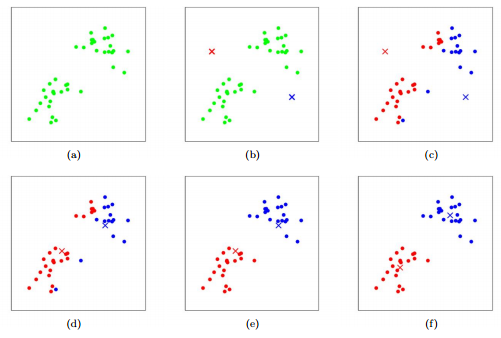
\includegraphics[scale=0.8]{Images/k-means-in-action.png}
    \caption{K-Means in action, original image from \cite{k-means-stanford-notes}}
    \label{fig:k-means}
\end{center}
\end{figure}

After a sufficient number of iterations, the results of the k-means algorithm will eventually converge. However, the algorithm will attempt to cluster data regardless of if it can be clustered or not. Therefore, K-means tends to perform more poorly on data that doesn't have a spherical shape. See Figure \ref{fig:k-means-complicated-shapes} for examples of k-means not performing well on complicated geometric shapes. 

\begin{figure}[H]
\begin{center}
    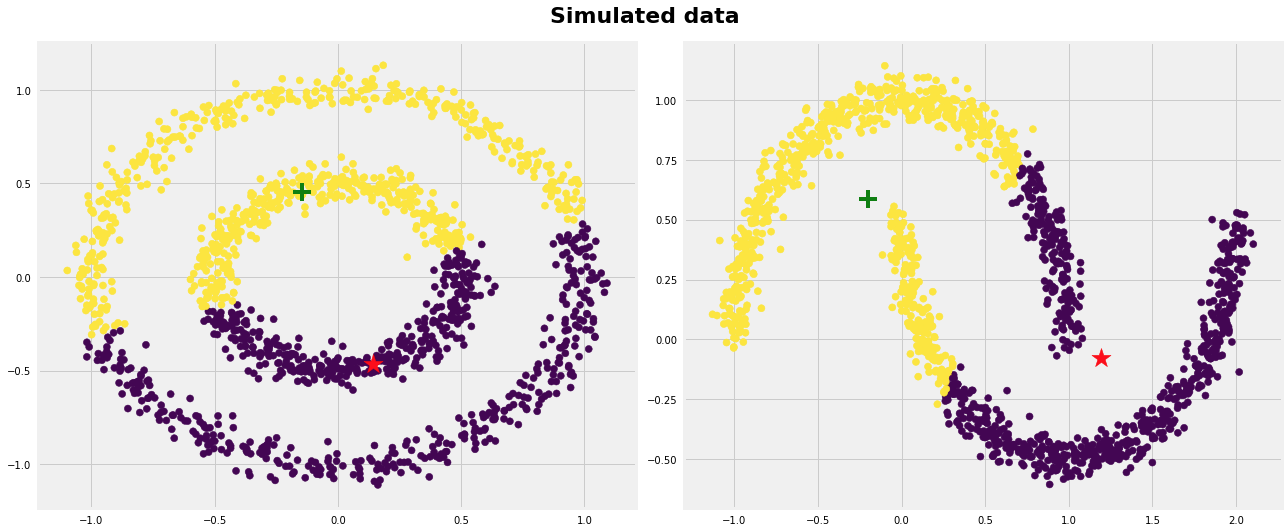
\includegraphics[width=\textwidth]{Images/k-means-complicated-shapes.png}
    \caption{K-Means performed on complicated geometric shapes, original image from \cite{k-means-towards-ds}}
    \label{fig:k-means-complicated-shapes}
\end{center}
\end{figure}

The k-means clustering algorithm uses a randomly generated seed to determine the starting centroids of the clusters. This inherent random nature of k-means can lead to the minimisation function getting stuck in a local minima. The `k-means++' initialisation scheme helps to mitigate this by initialising the centroids to be generally distant from each other, leading to provably better results than random initialisation. 

\subsubsection{Other clustering algorithms}

As a reader, based on the order you've presented this section in, I'd expect to see more than one clustering algorithm. Otherwise, there should be some evidence why you chose that particular algorithm.

\subsubsection{Cluster Quality Measures}
The two main methods of measuring the quality of a clustering are the \textit{Calinski-Harabasz} (CH) score and the \textit{Silhouette Coefficient} \cite{cluster-measures}.

The CH score \cite{ch-score}, also known as the Variance Ratio Criterion, is defined as the ratio between the within-cluster variance and the between-cluster variance (Equation \ref{eq:ch}). For a set of data of size $N$, which has been clustered into $k$ clusters:

\begin{equation}
    CH = \frac{SS_B}{SS_W}\times\frac{N-k}{k-1}
    \label{eq:ch}
\end{equation}
 
Where $SS_B$ is the overall between cluster variance, $SS_W$ is the overall within cluster variance, k is the number of clusters and N is the number of observations (Equation \ref{eq:ssb}). 

\begin{equation}
    SS_B = \sum_{i=1}^kn_i\vert\vert m_i - m\vert\vert ^2
    \label{eq:ssb}
\end{equation}

Where k is the number of clusters, $n_i$ is the number of observations in cluster $i$, $m_i$ is the centroid of cluster $i$, $m$ is the overall mean of the sample data, and $||m_i - m||$ is the $L^2$ norm (Euclidean distance) between the two vectors (Equation \ref{eq:ssw}).

\begin{equation}
    SS_W = \sum_{i=1}^k\sum_{x\in c_i} ||x-m_i|| ^ 2
    \label{eq:ssw}
\end{equation}
 
where $k$ is the number of clusters, $x$ is a data point, $c_i$ is the $i^{th}$ cluster, $m_i$ is the centroid of cluster $i$, and $||x-m_i||$ is the $L^2$ norm (Euclidean distance) between the two vectors. Well defined clusters have a large between cluster variance and a small within cluster variance. The higher the CH score, the better defined clusters the model has. \\

The Silhouette Coefficient \cite{silhouette-score} measures how similar that point is to other points in its cluster. It is bound between -1 and 1, where a higher score indicates that point $i$ is well matched to its cluster. If many points have a low or negative silhouette value, then the clustering solution might have too many or too few clusters. The silhouette coefficient for a single sample $i$ is composed of two scores whose mean then gives the overall silhouette coefficient score for that sample (Equation \ref{eq:silhouette}). 

\begin{equation}
    s(i) = \frac{b(i) - a(i)}{max\{a(i), b(i)\}}
    \label{eq:silhouette}
\end{equation}

where $a(i)$ is the average distance between data point $i$ and all other points in the same cluster and $b(i)$ is the average distance between data point $i$ and all other points in the next nearest cluster. Silhouette values can be used as a clustering evaluation criterion with any distance metric.

\subsection{Data Pre-processing: Outlier Analysis}

Talk about variance, standard deviation, Z-Score, what an outlier is.

\subsection{Transport for London APIs}
\label{section:tfl-api}

Across the entire London transport system there are over 19,000 bus stops, 700 bus routes, 8,000 buses and approximately 130,000 bus arrival predictions at any point in time \cite{tfl-bus-documentation}. However, Transport for London (TfL) does not provide an API that gives exact bus arrival times and so this information has to be inferred from the Countdown API which provides estimated arrival times \cite{tfl-api}.

\subsubsection{Countdown API}

The Countdown API provides real time predicted arrival times for buses in London. The expected arrival times are updated at the Countdown source every 30 seconds, so there is some room for error in regards to the inferred arrival time of the buses. This also means that there is no point in requesting information more frequently than every 30 seconds. \\

Depending on the request, the response can be made up of 5 different array types: \textit{Stop, Prediction, Flexible, Message} and \textit{URA Version} arrays. The sequence of these arrays in the response is undefined except that the \textit{URA Version} array always appears first. For the purpose of this project, the arrays that are relevant and will be returned are the \textit{URA Version} array and the \textit{Prediction} array. \\

An example request where Countdown was called for bus route 9 and stop code 490010357F (commonly known as "North End Road") can be seen in Figure \ref{fig:countdown-req}. The following parameters are set: 
\begin{itemize}
    \item stop code 2: the unique national identifier of the bus stop. Not to be confused with stop code 1 which is the public code for the bus stop displayed on the bus stop flag.
    \item line name: the route number displayed on the front of the bus.
\end{itemize}

\begin{figure}[H]
\begin{center}
    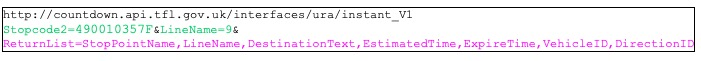
\includegraphics[keepaspectratio, width=17cm]{Images/countdown-req.jpg}
    \caption{Countdown API request}
    \label{fig:countdown-req}
\end{center}
\end{figure}

Figure \ref{fig:countdown-req} also demonstrates that users can choose what parameters Countdown should return in the response. For this project the following fields are set and returned in the \textit{Prediction} array: 
\begin{itemize}
    \item response type: this is returned by default and is always 1 for the \textit{Prediction} array.
    \item stop name: name of the bus stop.
    \item line name: the route number displayed on the front of the bus.
    \item direction id: 1 = outbound or 2 = inbound.
    \item destination text: the full length destination name of the trip the vehicle is on.
    \item vehicle id: the unique identifier of the vehicle.
    \item estimated arrival time: absolute time in UTC as per Unix epoch (in milliseconds).
    \item expiry time: time at which the corresponding prediction is no longer valid and should no longer be used. In this case it is the estimated arrival time + 30 seconds. 
\end{itemize}
The response also contains the timestamp that the response was processed in the \textit{URA Version} array. \\

The Countdown API returns a JSON of the form \texttt{[[URA array],[Prediction Array]]}. An example response where Countdown was called for bus route 9 and stop code 490010357F (commonly known as "North End Road") is seen in Table \ref{table:ura-array-stopa} and Table \ref{table:prediction-array-stopa} (the JSON information has been displayed in a table for ease of reading). Countdown was called at: Friday 15th May at 07:02:06 (time A).

\begin{table}[H]
    \centering
    \begin{tabular}{|c|c|c|}
        \hline
          Response Type & URA Version & Time that response was processed \\
        \hline
           4  & "1.0" & 1589526126913 \\
        \hline
        \end{tabular}
    \caption{\textit{URA Version} Array Route 9 at North End Road at Time A}
    \label{table:ura-array-stopa}
\end{table}

\begin{table}[H]
    \centering
    \setlength\tabcolsep{2pt}
    \begin{tabular}{|c|c|c|c|c|c|c|c|}
        \hline
          Response & Stop   &   Line & Direction & Destination & Vehicle & Estimated & Expiry \\[-3pt]
           Type & Name &    Name & ID &  Text & ID & Arrival &  Time \\
        \hline
             & "North &  &  &  &  & 158952 & 158952 \\[-3pt]
            1 & End Road" & "9" & 2 & "Aldwych" & 14510 & 6117000 & 6147000 \\
        \hline
             & "North &  &  &  &  & 158952 & 158952 \\[-3pt]
            1 & End Road" & "9" & 2 & "Aldwych" & 15448 & 6602000 & 6632000 \\
        \hline
        \end{tabular}
    \caption{\textit{Prediction Array} Route 9 at North End Road at Time A}
    \label{table:prediction-array-stopa}
\end{table}

When Countdown was called to give the expected arrival time on route 9 for "North End Road", it was also called at the same time to give the response for "Kensington Olympia Station". Table \ref{table:prediction-array-stopb} shows the \textit{Prediction Array} for bus route 9 and stop code 490008652A (commonly known as "Kensington Olympia Station"). Note that "Kensington Olympia Station" is the immediate station after "North End Road" in the 9 route to "Aldwych". Comparing Table \ref{table:prediction-array-stopa} and Table \ref{table:prediction-array-stopb}, it can be seen that the two same vehicles appear in both responses. This response can be interpreted visually as in Figure \ref{fig:countdown-response-timeA}.

\begin{table}[H]
    \centering
    \setlength\tabcolsep{2pt}
    \begin{tabular}{|c|c|c|c|c|c|c|c|}
        \hline
          Response & Stop   &   Line & Direction & Destination & Vehicle & Estimated & Expiry \\[-3pt]
            Type & Name &    Name & ID &  Text & ID & Arrival &  Time \\
        \hline
             & "Kensington &  &  &  &  & 158952 & 158952 \\[-3pt]
            1 & Olympia Station" & "9" & 2 & "Aldwych" & 14510 & 6169000 & 6199000 \\
        \hline
             & "Kensington &  &  &  &  & 158952 & 158952 \\[-3pt]
            1 & Olympia Station" & "9" & 2 & "Aldwych" & 15448 & 6654000 & 6684000 \\
        \hline
        \end{tabular}
    \caption{\textit{Prediction Array} Route 9 at Kensington Olympia Station at Time A}
    \label{table:prediction-array-stopb}
\end{table}

When Countdown is called again at Friday 15th May at 07:02:43 (time B) for both "North End Road" and "Kensington Olympia Station", the new response can be seen visually interpreted in Figure \ref{fig:countdown-response-timeB}. It can be seen that bus 14510 has now arrived at and passed "North End Road" and is on its way to "Kensington Olympia Station". This is indicated by the JSON response shown in Table \ref{table:prediction-array-stopa-updated} where bus 14510 is no longer returned in the \textit{Prediction Array} for Route 9 at "North End Road".

\begin{table}[H]
    \centering
    \setlength\tabcolsep{2pt}
    \begin{tabular}{|c|c|c|c|c|c|c|c|}
        \hline
          Response & Stop   &   Line & Direction & Destination & Vehicle & Estimated & Expiry \\[-3pt]
           Type & Name &    Name & ID &  Text & ID & Arrival &  Time \\
        \hline
             & "North &  &  &  &  & 158952 & 158952 \\[-3pt]
            1 & End Road" & "9" & 2 & "Aldwych" & 15448 & 6602000' & 6632000 \\
        \hline
        \end{tabular}
    \caption{\textit{Prediction Array} Route 9 at North End Road at Time B}
    \label{table:prediction-array-stopa-updated}
\end{table}

\begin{figure}[H]
\begin{center}
    \includegraphics[keepaspectratio, width=14cm]{Images/Countdown-response-timeA.png}
    \caption{Countdown API response at time A}
    \label{fig:countdown-response-timeA}
\end{center}
\end{figure}

\begin{figure}[H]
\begin{center}
    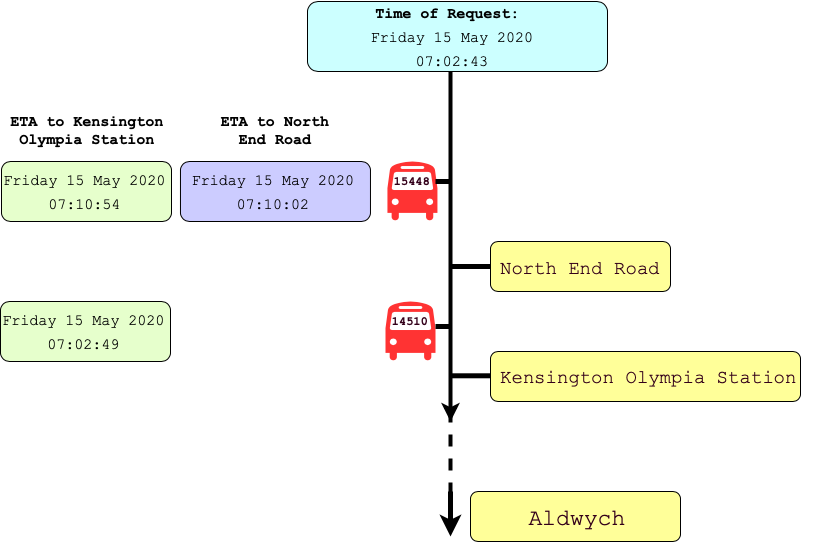
\includegraphics[keepaspectratio, width=14cm]{Images/Countdown-response-timeB.png}
    \caption{Countdown API response at time B}
    \label{fig:countdown-response-timeB}
\end{center}
\end{figure}

\subsubsection{Stoppoints API}

This API is called to give information on all bus stops for a particular route. A request takes the form:

\begin{center}
\texttt{https://api.tfl.gov.uk/line/bus\_route\_id/stoppoints}.
\end{center}

The response returns an array of stops. For each stop, information includes bus stop name, bus stop letter, all lines/routes serving that stop, facilities at the stop, including toilets, WiFi, phone number etc. and latitude and longitude. However, this API returns more stop ids than there actually are stops on a route. When put as parameters into the Countdown API call, some of the stop return estimated arrival times as expected, whereas others return HTTP errors. Therefore, it is useful to verify which stop ids are valid and which are invalid. 

\subsubsection{Stoppoints Sequence API}

This API is called to give the list of stops in the order that they are visited for a particular route. It can be called for both bus and underground routes. A request takes the form: 

\begin{center}
    \texttt{https://api.tfl.gov.uk/Line/bus\_route\_id/Route/Sequence/outbound}
\end{center}

For each of the stops returned in the list, the response also gives the interchanges with other lines and modes. The response also returns the latitude and longitude showing the path of the route so it can be plotted on a map.

\clearpage
